\chapter{Regularization Methods\label{cha:regularization}}
During the discussion of \vref{eq:optGoal} we have neglected the regularization
operator \(\mathcal{S} \from \mathbb{R}^d \to \mathbb{R}\).
This chapter starts with a short introduction to statistical regularization
theory and then compares two groups of regularization:
Tikhonov regularization and sparse regularization methods.

\section{Regularization Theory}
During the discussion of \vref{eq:optGoal} we have neglected the regularization
operator \(\mathcal{S} \from \mathbb{R}^d \to \mathbb{R}\).
Regularization helps us to train models that not only fit the data, but also generalize well.
To understand regularization, it is helpful to decompose our error functional.
Consider the expected prediction error at a point \(x\)~\cite{esl}:
\begin{align}
  \label{eq:bias-variance}
  \text{Pred. error}\left( x \right) = \Exp \left[ \left(y - \hat{f}(x) \right)^2 \right] &=
              \Bias\left[\hat{f}(x) \right]^2 + \Var\left[\hat{f}(x)\right] + \epsilon^2 \\
  \Bias \left[ \hat{f} (x) \right] &= \Exp \left[\hat{f}(x)\right] - f(x), \nonumber \\
  \Var \left[ \hat{f} (x) \right] &= \Exp \left[ \hat{f}(x) - \Exp \left[ \hat{f}(x) \right]^2 \right] \nonumber,
\end{align}
where \(\hat{f}(x)\) denotes our approximation of the real function \(f(x)\) and \(\mathbb{E}\) is the expected value of a random variable.
\sidetitle{Bias-Variance tradeoff}
\todo{What is bias/var/\(\epsilon\)?}
We call \cref{eq:bias-variance} the bias-variance tradeoff.
This equation splits the error into two different parts:
\begin{description}
\item[Bias] is the error caused by assumptions our model makes,
\item[variance] is the error caused by noise in the training data and
\item[irreduziable error (\(\epsilon\))] is the error caused by (what excactly?!).
\end{description}

Following the principle of \emph{Occam's razor} --- parsimonious models are better --- all regularization models penalize complexity.
Using regularization leads to smaller and simpler models, which increases the bias.
Of course, increasing this part of the error term makes no sense, if we would not get a payoff.
We use regularization methods to decrease the variance, thus making our model more robust to the possibly noisy data.
In this chapter we consider regularization methods that have both a scaling parameter, that controls the strenght of our assumptions, and (sometimes) parameters, that we use to modify the kind of our assumptions.
We call the parameter that controls the regularization strength \(\lambda\).

\sidetitle{Finding \(\lambda\)}
The choice of this parameter is important:
If we increase \(\lambda\), we exchange more bias for variance.
This is why \cref{eq:bias-variance} implies a tradeoff --- we cannot eat the cake and have it too!
We usually find the ideal \(\lambda\) by a more-or-less intelligent trial and error process.
To do this, we train a predictor for each \(\lambda\) we want to consider on a subset of our data (called the training set), and test its performance using either cross-validation or a seperate (holdout) validation set. 

\sidetitle{Prior Information}
Another way to reason about regularization is that it allow us to encode our
assumptions directly in the training process.
Many regularization methods --- and all mentioned in this chapter --- can be
viewed form a Bayesian perspective.

The choice of the regularization functional is crucial.
We do not know which one performs best a priori.
This is why we need to consider multiple methods, and evaluate their
effectiveness a posteriori.

In this chapter we are going to compare multiple choices and evaluate their effectiveness.
Each method encodes different assumptions, but all have in common that they
shrink our weights.

\section{Tikhonov Regularization}
\subsection{Theory}
We start with Tikhonov regularization, which is also called ridge regression in statistics.
Instead of solving an unconstrained minimization problem, we solve the following
problem:
\begin{align}\label{eq:tik-constrained}
 \text{minimize} \quad &
 \left\Vert  \bm{\Phi} \bm{\alpha} - \bm{y}  \right\Vert_2^2 \nonumber \\
\text{subject to} \quad &  \Vert \bm{\Gamma} \bm{\alpha}  \Vert_2 \leq l,
\end{align}
for a certain constant \(l\) and a linear operator \(\bm{\Gamma}\). 
By doing this we force our scaled weights to lie inside a \(d\)-dimensional sphere with a diameter of length \(l\).
To get a more convenient representation of~\cref{eq:tik-constrained} we use Lagrange multipliers to cast it into the equivalent Langrangian form
\begin{equation}\label{eq:tik-langrangian}
\mathcal{S} = \lambda \Vert \Gamma \bm{\alpha} \Vert_2^2.
\end{equation}
There is an one-to-one correspondence between \(l\) in~\cref{eq:tik-constrained} and \(\lambda\) in~\cref{eq:tik-langrangian}.
Both variables determine our constraints.
\todo{Explain what these constants do exactly.}
Tikhonov regularization fits into a Bayesian framework.
We can interpret it as a multivariate-Gaussian prior on the weights with zero mean and covariance matrix \(\bm{\Gamma}^{-1}\)~\cite{stat-inverse}.
The weights are therefore distributed as follows
\begin{equation*}
\alpha \sim \mathcal{N} (0, \bm{\Gamma}^{-1}).
\end{equation*}

A common choice for \(\Gamma\) is the identity matrix as proposed in~\cite{spatAdaptGrid}.
This correspond then to a penalty on the summed squared values of the weights.
It is a Gaussian prior with the identity as its covariance matrix.

\sidetitle{Diagonal Matrix}
Following the assumption of \vref{eq:coefficients-h2mix} we can express every function \(f\) in \(H_2^{\text{mix}}\) as a weighted sum of our basis functions.
For these functions the following upper bound on the hierachical coefficients \(\alpha_{\bm{l, i}}\) holds:
\begin{align}\label{eq:weights-bound}
  \vert \alpha_{\bm{l, i}} \vert &\leq 2^{-d -2 \vert \bm{l} \vert_1} \cdot \vert f \vert_{\bm{2}, \infty}\\
                             & = 2^{-d -2 \vert \bm{l} \vert_1} \cdot \Vert D^{\bm{2}} f \Vert_{\infty} \\
                              &\in \BigO \left( 2^{-2 \vert \bm{l} \vert_1} \right)
\end{align}
where the differential operator norm only depends on the function \(f\), and neither on the dimension nor the level of the basis functions~\cite{bungartzSparse}.
Because the dimension is constant for a given grid, we can treat it as a constant.

We can now use this fact to implement a regularization method that is better
suited for functions in \(H^2_\text{mix}\).
We impose an improved prior on the weights using Tikhonov regularization
with the matrix
\begin{equation}\label{eq:diagonal-prior}
\bm{\Gamma}_{i,i}^{1} = c^{\vert l \vert_1 - d},
\end{equation}
with a constant \(c\)
For \(c = 4\) this corresponds to a prior on the variance of the weights that is identical to the upper bound given by \cref{eq:weights-bound} up to a multiplicative constant.
We can also use a different \(c\), we can either treat it as a inherent constant
of the method or as an additional hyperparameter.
We use the dimension \(d\) as a normalizing factor, this way the prior
corresponds to the series \((1, \nicefrac{1}{4}, \nicefrac{1}{16}, \ldots)\).
The resulting series is depicted in \vref{fig:diagonal} for a two dimensional grid.

\begin{figure}[h]
  \begin{minipage}[c]{0.6\textwidth}
    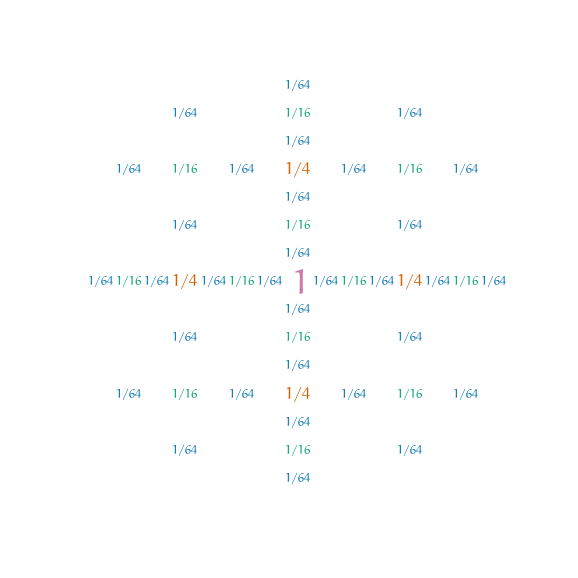
\includegraphics[width=\textwidth]{diagonal}
  \end{minipage}\hfill
  \begin{minipage}[c]{0.4\textwidth}
\caption[Diagonal Regularization]{
This figure shows the prior generated by \cref{eq:diagonal-prior} for a two
dimensional grid with level two. Each number is centered on a grid point and
corresponds to the prior for that particular weight.
}\label{fig:diagonal}
  \end{minipage}
\end{figure}

\subsection{Results \textit{\&} Discussion}
The diagonal method is awesome, because\ldots.

Consider the dataset with the predictors \(x_1, x_2\), both equally spaced
numbers in the interval \([0,1]\) and the target variable \(y\) defined by
\begin{equation*}
  y^p = 16x(1-x)y(1-y),
\end{equation*}
which is called the inverse parabola dataset.
\todo{Cite this function? Add contour plot.}
We know, that the surplusses that rise during sparse grid interpolation are equal to the bound defined by
\cref{eq:weights-bound}.
We assume, that the surplusses adhere to the prior~\ref{eq:diagonal-prior} for
sparse grid regression as well.
The following results were archived with the normal linear basis functions and a
grid with level 3.

\ldots

This is an indicator, that our prior can be useful at least for artificially
crafted data.
But does our prior improve the results for a function, when we only know the
variance of the weights?
To test this hypothesis, we construct an artificial dataset.
We first create a two dimensional sparse grid learner with level 3.
Let \(\bm{x} \in \mathbb{R}^{n \times 2}\) be a two dimensional feature vector,
where each row corresponds to one datum and is sampled from a two-dimensional
uniform distribution.
We then predict our target vector \(\bm{y}\) by predicting the result of
\(\bm{x}\).
We then add some gaussian noise with variance \(\sigma\).
Different values of \(\sigma\) are used, to craft variants of the same dataset,
with different signal-to-noise ratio.
Finally, we perform a bayesian optimization routine over some exponents \(c\)
and the regularization parameter \(\lambda\) for this dataset.
The results are shown in table \ldots.

We can see, that we archive a near-perfect error for the dataset with a
\textsc{SNR} x with \(c = 4\).
This verifies our hypothesis that the diagonal matrix regularization performs
better for a well-structured datasets.
Notice that for higher \textsc{SNRs}, we need a larger exponent base \(c\).
This indicates, that it might be helpful to include \(c\) as an additional
hyperparameter and not as a constant.

So far we have only seen examples for artificial datasets which adhere to our
assumptions by construction.
We now introduce our first real-world dataset, the concrete dataset.
\ldots.
We perform a grid search for a learner with level 4 for the diagonal
regularization with fixed exponent \(c = 4\) and for the standard ridge
regression.

\begin{figure}[htb]
  \centering
  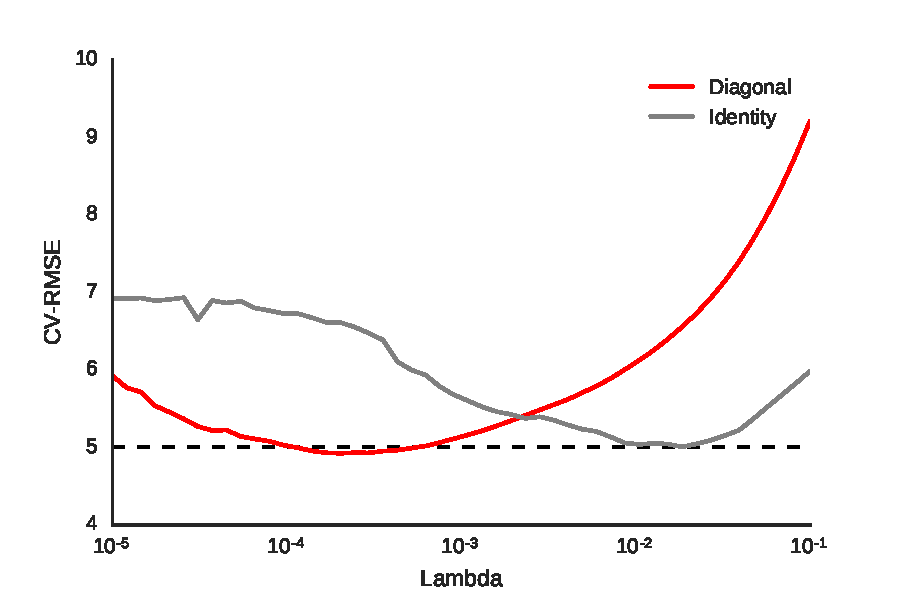
\includegraphics[width=\textwidth]{tikhonov_l4}
  \caption{Diagonal Matrix}
  \label{fig:tikhonov-l4}
\end{figure}

The results are shown in \cref{fig:tikhonov-l4}.
We can see that our method performs for this dataset better than the identity regularization.
Finally, we perform a bayesian optimization procedure for the same level, but include the exponent base \(c\) as a hyperparameter.
The results are compared in table \ldots.
We can see, that we archive the best performance for a c equal to \ldots, but
also that the diagonal method is an improvement over the identity functional,
even for a fixed \(c\).


\section{Sparse Regularization}
We have seen different variations of Tikhonov regularization.
All regularization methods so far have one thing in common: they used the squared Euclidian-norm.
In this section we are going to look at three different methods, which all use the Manhattan norm \(\Vert x \Vert_1  = \sum_i \vert x_i \vert\).

\sidetitle{The Lasso}
A first simple method is the so called lasso \footnote{In the original
  paper~\cite{lasso} the name lasso  was introduced as an
  acronym for ``least absolute shrinkage and selection operator''.
We use the term in a more metaphorical manner, where the lasso stands for an
actual rope used to catch cattle. See also~\cite{sparse-learning}.}
, first published by Tibshirani in his paper~\cite{lasso}. %coauthors?
We can represent this procedure in a form similiar to \cref{eq:tik-constrained} for a constant \(l\):
\begin{align}\label{eq:lasso-constrained}
\text{minimize} \quad &
 \left\Vert  \bm{\Phi} \bm{\alpha} - \bm{y}  \right\Vert_2^2 \\
\text{subject to} \quad & \Vert \bm{\alpha}  \Vert_1 \leq c,
\end{align}
which we can also cast into the more convenient Lagrangian representation
\begin{equation*}
\mathcal{S} = \lambda \Vert \bm{\alpha} \Vert_1.
\end{equation*}

We can also view this smoothness function from a Bayesian perspective.
In this context lasso regularization can be seen as a Laplace prior on the
weights with zero mean.
Another useful perspective is the geometric one. Lasso restricts our possible solutions to a hypercube with lenghts \(l\).
Both viewpoints lead to the same intutive result --- 
solutions where one variable is excactly zero are more likely to occur for the
lasso functional.
This leads to sparsity, i.e.~weight vectors with many entries that are zero.
% 1-norm closest to 0 norm (= feature selection), see lasso paper sec.10

\sidetitle{Elastic Net}
The lasso does not show good results in the following sitatuions~\cite{elasticnet}:
\begin{itemize}
\item In the (\(n < p\))-case the lasso selects at most \(n\) predictors.
\item Compared to the lasso, it handles highly-correlated predictors better.
While the lasso selects one of the predictors at random, or shows otherwise
unstable behavior, the ridge portion of the elastic net penalty has a
stabilizing effect on the coefficient path.
\item The Tikhonov regression shows better practical results than the lasso in the
  correlated case.
\end{itemize}
All those reasons indicate, that the lasso is not a good choice for many problems.
The Tikhonov regression is no direct competitor, because it lacks the increased interpretability of the sparse methods.
We now discuss an alternative regularization methods, that is a combination of
the lasso and the Tikhonov functionals: the elastic net.
It was first introduced in~\cite{elasticnet} by \citeauthor{elasticnet}.

The elastic net functional is given by
\begin{equation}
  \label{eq:elastic-net}
  \mathcal{S}(\bm{\alpha}) = \lambda \Vert \bm{x} \Vert_2 +  \gamma \Vert \bm{x} \Vert _1,
\end{equation}
where \(\lambda\) and \(\gamma\) are two independent parameters~\cite{elastic-net}.
Although this form is more convenient for the following calculations, it is not intuitively useful for actual usage.
We can reparametrize the previous equation as
\begin{equation*}
  \mathcal{S}(\bm{\alpha}) = \lambda_1 \left\{ \left(1 - \lambda_2 \right) \Vert \bm{x} \Vert_2  + \lambda_2 \Vert \bm{x} \Vert _1\right\},
\end{equation*}
where \(\lambda_1\) determines the overall regularization effect and \(\lambda_2\) controls the relative influence of the lasso term.
From this equation we can recover both the Ridge and the lasso\ regularization, by setting \(\lambda_2\) to \(0\) or \(1\) respectively.
\todo{Show prior and constraint region.}
% Maybe show coefficient path?

\sidetitle{Group Lasso}
Another useful generalization of the lasso is the grouped lasso that shrinks
groups of weights at the same time.
It was first developed by \citeauthor{grouplasso} in~\cite{grouplasso}, then
extended to the logistic regression method in~\cite{grouplasso-logistic}.
\citeauthor{grouplasso-generalizations} discussed some generalizations of the
method in~\cite{grouplasso-generalizations} and a discussion of the statistical
properties is offered by~\cite{grouplasso-benefit}.
The discussion here follows~\cite{sparse-learning}, unless otherwise noted.

Let \(\mathcal{P}\) denote a partition of \(\bm{\alpha}\), i.e.~a set of disjoint subsets whose union is \(\bm{\alpha}\).
We can then define the group lasso as
\begin{equation*}
  \mathcal{S}({\bm{\alpha}}) = \lambda \sum_{p \in \mathcal{P}} \left(\sqrt{\vert p \vert}\right) \Vert  p \Vert_2,
\end{equation*}
where \(\vert p \vert\) denotes the cardinality of \(p\) and is used as a weighting factor.
We can choose different weights for the group, but the square root of the cardinality is a useful factor that is simple to calculate and works well in practice.
If we would not include this factor, larger groups would be more likely to be included in the final model.

We partition our weights in the following way:
The first group is the bias term, the second family of groups is composed of the grid points which are constant for all dimensions but one, the second family is composed of the grid points which are constant for all but two dimensions (first order interaction terms), and so on.
This grouping corresponds to classical feature selection, where we treat each dimension as a feature, and each interaction between features as a new interaction feature.
Note that by choosing partitions of size one we can recover the original lasso penalty.

The lasso functional --- and thus also the elastic net smoothness term --- is not differentiable at zero.
We were able to solve the Tikhonov regularization method using a standard conjugated gradient scheme, this is not possible for the methods presented in this section.
We cannot rely on gradient information anymore, we need to solve this problem using a gradient-free optimization procedure.
This does not mean, that we have to use a black-box-optimization algorithm.
We can still profit from the structure of our problem.
In the following section we present a solver for least-squares problems that are regularized with either the lasso or the elastic net. 
\subsection{Proximal Methods}
There are many solvers for the lasso and related methods.
In this section we present the Fast Iterative Shrinkage Tresholding Algorithm (\fista), first introduced in~\cite{fista}.
This solver offers a good compromise between flexibility and performance and we
can use it to solve all presented sparse regularization methods.
The discussion of \fista\ follows~\cite{fista}, the description of
the proximal operators follows~\cite{proxsurvey}.
\fista\ is able solve problems of the form
\begin{equation}\label{eq:composite-goal}
\min_{\bm{\alpha}} F(\bm{\alpha}) = f(\bm{\alpha}) + g(\bm{\alpha}),
\end{equation}
i.e.~minimizing functions that can be expressed as a sum of a convex, smooth function \(f(\bm{\alpha})\) and another convex, possibly non-smooth function \(g(\bm{\alpha})\).
\sidetitle{Lipschitz constant}
It is required that \(f(\bm{\alpha})\) has a Lipschitz-continuous gradient. 
This means that the following condition holds for all possible vectors \(\bm{x}\) and \(\bm{y}\) for some positive constant \(L\):
\begin{equation}   \label{eq:lipschitz}
 \Vert \bm{\nabla} f(\bm{x}) - \bm{\nabla} f(\bm{y}) \Vert \leq L \Vert \bm{x} - \bm{y} \Vert.
\end{equation}
We call the smallest possible value of \(L\) the Lipschitz constant.

For our goal given by \cref{eq:composite-goal} we set \(f(\bm{\alpha})\) to
\begin{equation*}
 f(\bm{\alpha}) = \frac{1}{2} \left\Vert  \bm{\Phi} \bm{\alpha} - \bm{y}   \right\Vert_2^2,
\end{equation*}
such that the gradient of \(f\) is then given by
\begin{equation*}
  \bm{\nabla} f(\bm{\alpha}) = \bm{\Phi}^\intercal \left(\bm{\Phi} \bm{\alpha} - \bm{y} \right).
\end{equation*}
The Lipschitz constant for the gradient of \(f\) is
\begin{equation}
  \label{eq:lipf}
  L_{\bm{\nabla} f} = {\left(\sigma_{\max} \left(\bm{\Phi}\right)\right)}^2,
\end{equation}
where \(\sigma_{\max} \) corresponds to the maximum singular value~\autocite{fista}.
Additionally we set \(g\) to
\begin{equation*}
  g(\bm{\alpha}, \lambda) = \mathcal{S} \left( \bm{\alpha}, \lambda \right).
\end{equation*}

\sidetitle{Moreau envelope}
We now define the Moreau envelope of a function \(g (\bm{\alpha})\), which is given for any \(\lambda \in (0, +\infty)\) by
\begin{equation}
  \label{eq:moreau-reg}
  M_{g}(\bm{\alpha}, \lambda) = \inf_{\bm{x}} \left\{  g(x) + (1/(2\lambda)) \Vert x - \bm{\alpha} \Vert_2^2 \right\}.
\end{equation}
It is a regularized, smooth version of our function \(g(\bm{\alpha})\) that has the
same minimum as \(g(\bm{\alpha})\).
That means, that every point that minimizes \(M_{g}(\bm{\alpha}, \lambda)\) also
minimizes our original function \(g (\bm{\alpha})\)~\cite{proxsurvey}.
Finally, we are able to define the proximal operator that returns the infimum
point of \cref{eq:moreau-reg} by
\begin{equation}
  \label{eq:proximal}
  \prox[\(g\)]{\bm{\alpha}}{\lambda}= \argmin_{\bm{x}} \left\{ g (\bm{x}) + (1/ (2 \lambda)) \Vert \bm{x} - \bm{\alpha} \Vert_2^2 \right\}.
\end{equation}
\sidetitle{Proximal Operator}
The proximal operator can be viewed as a gradient step with stepsize \(\lambda\) on the Moreau envelope
\(M_g(\bm{\alpha}, \lambda)\)
\begin{equation*}
  \prox[\(g\)]{\bm{\alpha}}{\lambda} = \bm{\alpha} - \lambda \bm{\nabla} M_{g}(\bm{\alpha}, \lambda).
\end{equation*}
This identity follows by rewriting \cref{eq:moreau-reg} in terms of the proximal operator and calculating the gradient~\cite{proxsurvey}.
We can use \cref{eq:proximal} to minimize \(M_g(\bm{\alpha}, \lambda)\) and
thus also for optimizing \(g(\bm{\alpha})\).
In the most general case \cref{eq:proximal} would imply the need to solve a convex optimization problem.
Fortunately we can find closed form solutions for many functions.
Consider for example \(g(\bm{\alpha}) = 0\).
In this case the Moreau envelope and the proximal operator are trivial
\begin{align*}
 M_{0}(\bm{\alpha}, \lambda) &= \inf_{\bm{x}} \left\{ 0 + 1/(2 \lambda) \Vert \bm{\alpha} - \bm{x} \Vert_2^2 \right\}, \\
 \prox[\(0\)]{\bm{\alpha}}{\lambda} &= \bm{\alpha}.
\end{align*}
It is obvious that the minimum of \(M_g(\bm{\alpha}, \lambda)\) is equivalent to the minimum of \(g(\bm{\alpha})\), the proximal operator is corresponds to a gradient step on \(M_g\).

We are now going to develop a minimizer for our composite goal that resembles a majorization-minimization algorithm.
To do this, we first define an upper-bound of \(F(\bm{\alpha})\)~(\emph{majorizing}) that we are then going to minimize~(\emph{minimization})~\autocite{proxsurvey}.

\sidetitle{Upper Bound}
We first give a regularized linearization of \(f(\bm{\alpha})\) at an arbitrary,
but fixed point \(\bm{y}\) for an \(L > 0\):
\begin{equation}\label{eq:f-approx}
  \hat{f}_L(\bm{\alpha}, \bm{y}) = f(\bm{y}) + \left< \bm{\alpha} - \bm{y}, \bm{\nabla} f (\bm{y}) \right> +
  L/2 \Vert \bm{\alpha} - \bm{y} \Vert_2^2,
\end{equation}
where the angle brackets \( \left< \bm{x}, \bm{y} \right> = \bm{y}^\intercal \bm{x} \) represent the inner product.
The first two summation terms are given by the first order Taylor expansion of \(f(\bm{\alpha})\) at the point \(\bm{y}\), the last term can be interpreted as a trust-region or regularization, that punishes large deviations from~\(\bm{y}\)~\cite{proxsurvey}.
We then combine this linearization with our second function to archive an upper-bound of \(F(\bm{\alpha})\):
\begin{equation}\label{eq:goal-approx}
  Q_L(\bm{\alpha}, \bm{y}) = f(\bm{y}) + \left< \bm{\alpha} - \bm{y}, \bm{\nabla} f (\bm{y}) \right> +
  L/2 \Vert \bm{\alpha} - \bm{y} \Vert_2^2 +
  g(\bm{\alpha}).
\end{equation}
We can see from \cref{eq:lipschitz} that \(Q_L(\bm{\alpha}, \bm{y})\) is an
upper-bound of \(F(\bm{\alpha})\) iff.~L is equal to or greater than the Lipschitz
constant of \(\bm{\nabla} f(\bm{\alpha})\).

\sidetitle{Fixed-point minimizer}
The minimizer for this approximation is then given as the fixed-point equation
\begin{align}\label{eq:step}
  \pi_{g(\bm{\alpha})}(\bm{\alpha}^*, L) &=  \argmin_{\bm{x}} \left\{ Q_L(\bm{x}, \bm{\alpha}) \right\}\nonumber\\
       &= \prox[\(g\)]{\bm{\alpha^*} - L^{-1} \bm{\nabla} f (\bm{\alpha^*})}{L^{-1} } \nonumber\\
       &= \prox[\(g\)]{\bm{\alpha^*} - L^{-1} \bm{\Phi}^\intercal \left(\bm{\Phi} \bm{\alpha^*} - \bm{y} \right)}
         {L^{-1}},
\end{align}
where \(\bm{\alpha}^*\) denotes the optimal solution and \(L\) is the Lipschitz constant of \(\bm{\nabla} f\) given by \cref{eq:lipf}~\cite{fista}.
In this equation \(L\) is used to determine the optimal stepsize.
This minimizer is called proximal gradient algorithm (or proximal-splitting) in the literature, because we first perform a gradient step on \(f'_L(\bm{\alpha})\) given by~\ref{eq:f-approx} and then a proximal step on \(g(\bm{\alpha})\)~\cite{proxsurvey}.
Using \cref{eq:step} repeatedly on a point will result in the fixed-point, i.e.~the minimum of the upper bound, and thus also in the minimum of our original goal~\cite{proxsurvey}.

\begin{algorithm}
 \caption{Iterative Shrinkage Tresholding Algorithm (\ista)~\cite{fista}}\label{alg:ista} 
 \begin{algorithmic}[1]
   \Require{Lipschitz constant \(L\) of \(\bm{\nabla} f\), regularization parameter \(\lambda\)}
    \Statex
    \Function{Ista}{$L, \bm{\alpha}$} \Comment{\(\bm{\alpha}\) is an initial guess}
      \While{not converged}
        \Let{$\bm{\alpha}$}{\( \pi_{g(\bm{\alpha})} \left( \bm{\alpha}, L \right) \)}
      \EndWhile
     \State \Return{\(\bm{\alpha}\)}
    \EndFunction
\end{algorithmic}
\end{algorithm}

\Cref{eq:step} is all we need to define the simple iterative scheme called
Iterative Shrinkage Tresholding Algorithm~(\ista) as seen in \cref{alg:ista}.
Originally the name \ista\ was only used for solving the Lasso problem, but is now used for the more general algorithm as well. 
For our trivial function \(g(\bm{\alpha}) = 0\) this iterative scheme is identical to the standard gradient descent algorithm.

\sidetitle{Proximal Operators for Regularization}
So far we have only seen the proximal operator of a very simple function.
This is of course not satisfactory, the motivation for this chapter is solving the Lasso and the Elastic Net regularization problems.
Fortunately, closed form solutions for the other needed proximal operators exist as well:
\begin{align}
\label{eq:prox-lasso}
\text{for Lasso} \quad &&
    \left( \prox[\(\lambda \Vert \bm{\alpha} \Vert_1\)]{\bm{\alpha}}{t} \right)_i &= \left[\alpha_i - t \lambda \right]_+
    - \left[ -\alpha_i - t \lambda \right]_+, \\
\text{for Ridge} \quad &&
                          \left(  \prox[\( \lambda \Vert \bm{\alpha} \Vert_2^2\)]{\bm{\alpha}}{t} \right)_i &= (\alpha_i/(1 + 2t \lambda)), \nonumber\\
  \text{for Elastic Net} \quad && \prox[\( \lambda \Vert \bm{\alpha} \Vert_1 + \gamma \Vert \bm{\alpha} \Vert_2^2\)]{\bm{\alpha}}{t} &=
                                                                                                                                       \left( 1/(1 + 2 t \gamma) \right) \left(\prox[\(\lambda \Vert \bm{\alpha} \Vert_1\)]{\bm{\alpha}}{t}\right) \nonumber\\
  \text{for Group Lasso} \quad && {\left(\prox[\( \lambda \sum_{p \in \mathcal{P}} \sqrt{\vert p \vert} \Vert p \Vert_2 \)]{\bm{\alpha}}{t} \right)}_p &=
                                                                                     \left[ 1 - \left(\lambda t \sqrt{\vert p \vert}\right) \left( \Vert p \Vert_2 \right)^{-1} \right]_+ p \nonumber
\end{align}
where \( \left( x \right)_+ = \max(x, 0) \) denotes the positive part of \(x\)
and \(t\) is a stepsize.
The regularization parameters depend on the function \(g(\bm{\alpha})\).
We omit the derivations for the sake of brevity, the interested reader refers to the survey paper~\cite{proxsurvey}.
By setting the regularization parameter \(\lambda\) equal to zero, we again recover the gradient minimization method.

\sidetitle{Minimizing Lasso}
These proximal operators can be used to define a minimizer for a non-smooth
function \(g\).
For example, combining~\cref{eq:step} with the proximal operator for the
Lasso functional \(g(\bm{\alpha}) = \lambda \Vert \bm{\alpha} \Vert_1\) given by~\cref{eq:prox-lasso} results in
the minimizer
\begin{align*}
  \pi_{\lambda \Vert \bm{\alpha} \Vert_1}(\bm{\alpha^*} ,L)
  &=  \prox[\(\lambda \Vert \bm{\alpha} \Vert_1\)]{\bm{\alpha^*} - L^{-1} \bm{\nabla} f (\bm{\alpha^*})}{L^{-1}} \\
  &= {\left[ \left(\bm{\alpha^*} - L^{-1} \bm{\nabla} f (\bm{\alpha^*}) \right) - \lambda L^{-1} \right]}_+ -
    {\left[ -\left(\bm{\alpha^*} - L^{-1} \bm{\nabla} f (\bm{\alpha^*}) \right) - \lambda L^{-1} \right]}_+,
\end{align*}
again given as a fixed-point iteration.
In this equation the function \( \left[ x \right]_+ \) is applied element-wise on its input vector.
We can then use this minimizer with \cref{alg:ista} to compute a solution to
the Lasso problem.
The fixed-point equations for the Lasso and Elastic Net Regularization are
computed analogously.

\sidetitle{Nesterov's accelerated gradient descent}
\ista always converges to the global maximum, but only does so linearly~\cite{fista}.
To overcome this problem, Beck and Teboulle combined the \ista algorithm with
the accelerated gradient descent algorithm discovered by Nesterov. 
Nesterov's accelerated gradient descent is closely related to the ordinary
gradient descent algorithm.
The first step is identical, each following step carries some momentum of the
step before, thus stabilizing the procedure.
It is an optimal first-order optimization schema, i.e.~one that cannot be
improved asymptotically.
It archives quadratic convergence.
This property is retained when combined with the proximal-splitting procedure \cref{alg:ista}, the result is called \fista~\cite{fista}.
Each step of \fista\ evaluates the gradient and the proximal operator once, just as \ista does.
This means that the accelerated algorithm has a comparable cost for each iteration.

\sidetitle{Linesearch}
Another problem with \cref{alg:ista} is its dependence on the Lipschitz constant of
\(\bm{\nabla} f\) to determine the optimal stepsize.
For our choice of \(f\), the best constant \(L\) is given by~\cref{eq:lipf}.
To avoid this expensive calculation, we use a backtracking line search to
determine a suitable stepsize.
In this line search procedure we use \cref{eq:goal-approx} as an upper bound for \cref{eq:composite-goal}.
We do this by iterating and finding the smallest \(L\) for which
\cref{eq:goal-approx} is an upper bound.
This always results in the Lipschitz constant~\cite{fista}.
It is then straightforward to derive \cref{alg:linesearch}.

\begin{algorithm}[h!]
 \caption{Linesearch~\cite{fista}}\label{alg:linesearch}
 \begin{algorithmic}[1]
  \Require{\(L > 0, \eta > 1, \bm{\alpha}\)} 
  \Statex
  \Function{Linesearch}{$\bm{\alpha}, L$}
    \Let{\(i\)}{\(0\)}
    \Do
      \Let{L}{\(\eta^i L\)}
      \Let{prox}{\(\pi_{\bm{\alpha}} (\bm{\alpha}, L)\)}
      \Let{\(i\)}{\(i + 1\)}
    \doWhile{$F(\text{prox}) < Q_L(\text{prox}, \bm{\alpha})$}
    \State \Return{prox and \(L\)} \Comment{Also return prox to avoid duplicate calculations.}
  \EndFunction
 \end{algorithmic}
\end{algorithm}

We need to evaluate the line search once for each iteration step.
It is possible that this procedure finds a non-optimal \(L\), i.e.~an \(L\) that
is larger than the Lipschitz constant.
This leads to a smaller stepsize, which is not a problem in practice, because
our optimization procedure still converges, although slower than possible.
We have to take that into consideration for our choice of linesearch parameters.
Usual values are \(L = 0.5\) and~\(\eta = 2\).
Using \cref{alg:linesearch} we can finally present an optimal first order optimization algorithm, shown by \cref{alg:fista}.

It is of course possible to use a constant stepsize like in \cref{alg:ista}.
To do this, replace the line search with the minimal value of \(L\) and
calculate \(\pi(\bm{\alpha}, L)\) directly.
We can also integrate the linesearch into the \ista algorithm, by replacing the
fixed \(L\) with a call to the linesearch subroutine.
A comparison of the practical speed of \ista and \fista with constant stepsize can be seen in~\cref{fig:fista-convergence}.

An alternative backtracking scheme for \fista is offered in~\cite{fista-backtracking}.
It offers the same asymptotic convergence speed, but shows practical improvements for some minimization problems.

\begin{figure}[bt]
  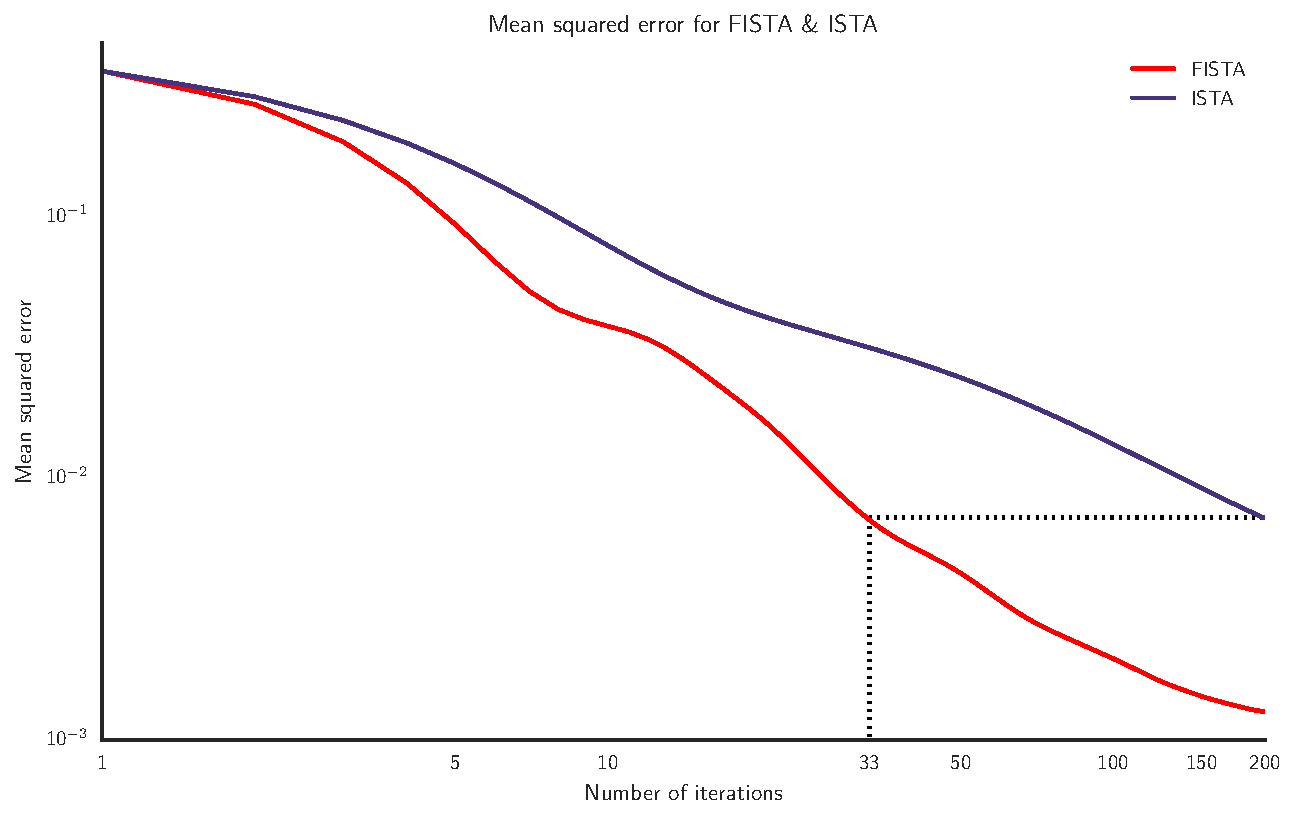
\includegraphics[width=\textwidth]{fista}
  \caption[Comparison of \fista and \ista]{Comparison of \fista and \ista, both with constant stepsize.
    The figure shows the training \textsc{mse} for 500
    iterations with \(\lambda = 0.1\) for the training set of the concrete
    data set.
    The dotted lines indicate the best value reached by \ista.
    Note that \fista is able to return a better result after only 56
    iterations ---
    compared to the 500 needed by \ista.
  }\label{fig:fista-convergence}
\end{figure}

\begin{algorithm}[h]
 \caption{Fast Iterative Shrinkage Tresholding Algorithm (\fista)~\cite{fista}}\label{alg:fista} 
 \begin{algorithmic}[1]
   \Require{Initial guess for Lipschitz constant \(L\) of \(\bm{\nabla} f\), regularization parameter \(\lambda\)}
    \Statex
    \Function{Fista}{$L, \bm{\alpha}$} \Comment{\(\bm{\alpha}\) is an initial
      guess for \(\alpha^*\).}
      \Let{\(\bm{y}\)}{\(\bm{\alpha}\)}
      \Let{\(t\)}{\(1\)}
      \While{not converged}
        \Let{\(\bm{\alpha}_{\text{before}} \)}{\(\bm{\alpha}\)}
        \Let{$\bm{\alpha}, L$}{\Call{Linesearch}{$ \bm{y}, L$ }} \Comment{Linesearch returns \(\pi_L (\bm{y})\) and the used L.}
        \Let{\(t_\text{before}\)}{\(t\)}
        \Let{\(t\)}{\(\nicefrac{1}{2} (1 + \sqrt{1+4t^2}) \)}
        \Let{\(\bm{y}\)}{\(\bm{\alpha} + \left( t_\text{before} -1 \right) t^{-1} 
                    \left(\bm{\alpha} - \bm{\alpha}_{\text{before}} \right)\)}
      \EndWhile
     \State \Return{\(\bm{\alpha}\)}
    \EndFunction
\end{algorithmic}
\end{algorithm}

%%% Local Variables:
%%% mode: latex
%%% TeX-master: "../main"
%%% End:


\section{Implementation}

\tikzumlset{fill class = white, fill template = white, fill package = white}

\begin{figure}[h]
  %https://tex.stackexchange.com/questions/140739/extending-figures-into-the-margin-on-even-vs-odd-pages
 \makebox[0.9\textwidth][l]{\begin{tikzpicture}
    \begin{umlpackage}{RegularizationFunctions}
      \umlclass[type=abstact, x=1]{RegularizationFunction}{
      }{
        \umlvirt{+ eval(weights : DataVector) : double}\\
        \umlvirt{+ prox(weights : DataVector, stepsize : double) : DataVector}
      }

      \umlclass[y=0, x=10]{ZeroFunction}{}{
        + ZeroFunction()
      }

      \umlclass[y=6, x=0]{RidgeFunction}{
        - lambda : double
      }{
       + RidgeFunction(lambda : double)}

      \umlclass[y=-4, x=0]{LassoFunction}{
        - lambda : double
      }{
      + LassoFunction(lambda : double)}

      \umlclass[y=-4, x=10]{ElasticNetFunction}{
        - lassoFunc : LassoFunction \\
        - lambda1 : double\\
        - lambda2 : double
      }{
        + ElasticNetFunction(lambda : double, l1Ratio : double)
      }

      \umlclass[y=5, x=10]{GroupLassoFunction}{
        - lambda : double\\
        - groups : map<coords, int>\\
        - storage : gridStorage*\\
        - groupIx : map<int, index>\\
        - lastSize: int
      }{
        + GroupLassoFunction(lambda : double,\\
        \phantom{+ } storage : GridStorage*)\\
        - calculateNorm(weights : DataVector) : DataVector\\
        - calculateIndices(weights : DataVector) : void
      }

    \umlinherit[]{ZeroFunction}{RegularizationFunction} 
    \umlinherit[]{RidgeFunction}{RegularizationFunction} 
    \umlinherit[]{LassoFunction}{RegularizationFunction} 
    \umlinherit[]{ElasticNetFunction}{RegularizationFunction} 
    \umlinherit[]{GroupLassoFunction}{RegularizationFunction} 

    \umlassoc{LassoFunction}{ElasticNetFunction}
    \end{umlpackage}
  \end{tikzpicture}}
  \caption[Class diagram for RegularizationFunctions]{Implementation of
    RegularizationFunctions}
\label{fig:uml-regularization}
\end{figure}
% \begin{tikzpicture}
%   \begin{umlpackage}[x=0, y=0]{Fista}
%     \umlclass[type=abstact, width=20ex]{sgpp::solver::FistaBase}{
      
%     }{
%         {\itshape + solve(op : OperationMultipleEval, \\\phantom{+ solve} weights : DataVector,
%         y : DataVector,\\\phantom{+ solve} maxIt : size\_t, threshold : double) : void}
%     }

%     \umlclass[template={F}, y=-4, name=Fista]{sgpp::solver::Fista}{
%     - regularizationFunction : F 
%     }{
%       + Fista( regularizationFunction : F)\\
%       + solve(op : OperationMultipleEval, \\\phantom{+ solve} weights : DataVector,
%         y : DataVector,\\\phantom{+ solve} maxIt : size\_t, threshold : double) : void
%     }
       
%     \umlinherit[]{sgpp::solver::FistaBase}{sgpp::solver::Fista}
%   \end{umlpackage}
% \end{tikzpicture}

As seen in the class diagram above, \fista is implemented as a templated class
that determines the used function \(g\).
The template allows the compiler to inline all calls to prox and eval, which get
evaluated once during each iteration.
Even though the implementation of \fista is split into various subroutines, they
all get inlined into one efficient loop.
We have to use a baseclass, otherwise we would not be able to attain a pointer
to the Fista class, without knowing the used type of regularization.

\subsection{Results \textit{\&} Discussion}
We can calculate the value of \(\lambda\) for which all weights are exactly
zero, using the method developed by \citeauthor{regularizationpaths} in~\cite{regularizationpaths}.
The maximum \(\lambda\) is given by
\begin{equation*}
  \lambda_{\text{max}} = \frac{\max_i \vert \langle \bm{\Phi}_i, \bm{y} \rangle \vert}{\lambda_2},
\end{equation*}
where the index \(i\) denotes the \(i\)th column of the matrix, and
\(\lambda_2\) the amount of \(l_1\) regularization.
We then construct a logarithmic grid starting with \(\lambda_{\text{max}}\) to
\(\lambda_{\text{min}} = \varepsilon \lambda_{\text{max}}\), where
\(\varepsilon\) is typically set to 0.001.
It is more efficient to start the path with all weights set to zero, see~\cite{regularizationpaths} for a more advanced discussion.

We introduce our first dataset, the Friedman1 dataset, first published
in~\cite{datasets-friedman}.
Let \(\bm{x}^F = (x_1, \ldots, x_{10}) \in \mathbb{R}^{10}\) be a uniformally distributed vector.
We use \(\bm{x}\) as our predictors, and define
\begin{equation}\label{eq:friedman1}
  y = 10 \sin(\pi x_1 x_2) + 20(x_3 - 0.5)^2 + 10x_4 + 5x_5 + \varepsilon,
\end{equation}
with \(\varepsilon \sim \mathcal{N}(0,1)\) as additional gaussian noise.
We perform some preprocessing steps on this dataset, these can be found in \cref{sec:friedman}.
This dataset has many useful properties, we will use it throughout this thesis.
The fact that the optimal error is given by the normal noise variance is
helpful, to determine the performance of this method.

%%% Local Variables:
%%% mode: latex
%%% TeX-master: "../main"
%%% End:

